\documentclass[twoside,a4paper]{article}
\usepackage{geometry}
\geometry{margin=1.5cm, vmargin={0pt,1cm}}
\setlength{\topmargin}{-1cm}
\setlength{\paperheight}{29.7cm}
\setlength{\textheight}{25.3cm}

% useful packages.
\usepackage{amsfonts}
\usepackage{amsmath}
\usepackage{amssymb}
\usepackage{amsthm}
\usepackage{enumerate}
\usepackage{graphicx}
\usepackage{multicol}
\usepackage{fancyhdr}
\usepackage{layout}

% some common command
\newcommand{\dif}{\mathrm{d}}
\newcommand{\avg}[1]{\left\langle #1 \right\rangle}
\newcommand{\difFrac}[2]{\frac{\dif #1}{\dif #2}}
\newcommand{\pdfFrac}[2]{\frac{\partial #1}{\partial #2}}
\newcommand{\OFL}{\mathrm{OFL}}
\newcommand{\UFL}{\mathrm{UFL}}
\newcommand{\fl}{\mathrm{fl}}
\newcommand{\op}{\odot}
\newcommand{\Eabs}{E_{\mathrm{abs}}}
\newcommand{\Erel}{E_{\mathrm{rel}}}

\begin{document}

\pagestyle{fancy}
\fancyhead{}
\lhead{NAME Jiatu Yan}
\chead{Numerical Analysis homework \#6}
\rhead{Date 2020.5.17}


\section*{I. \small{Calculate the three function in the interval $[0.99, 1.01]$.} }

We can see that each function have the values very close to zero 
in the interval $[0.99, 1.01]$, but their errors are different.

I multiplied the values of each function by $10^{14}$ to magnify the scale.
\begin{figure}[ht]
        \centering
        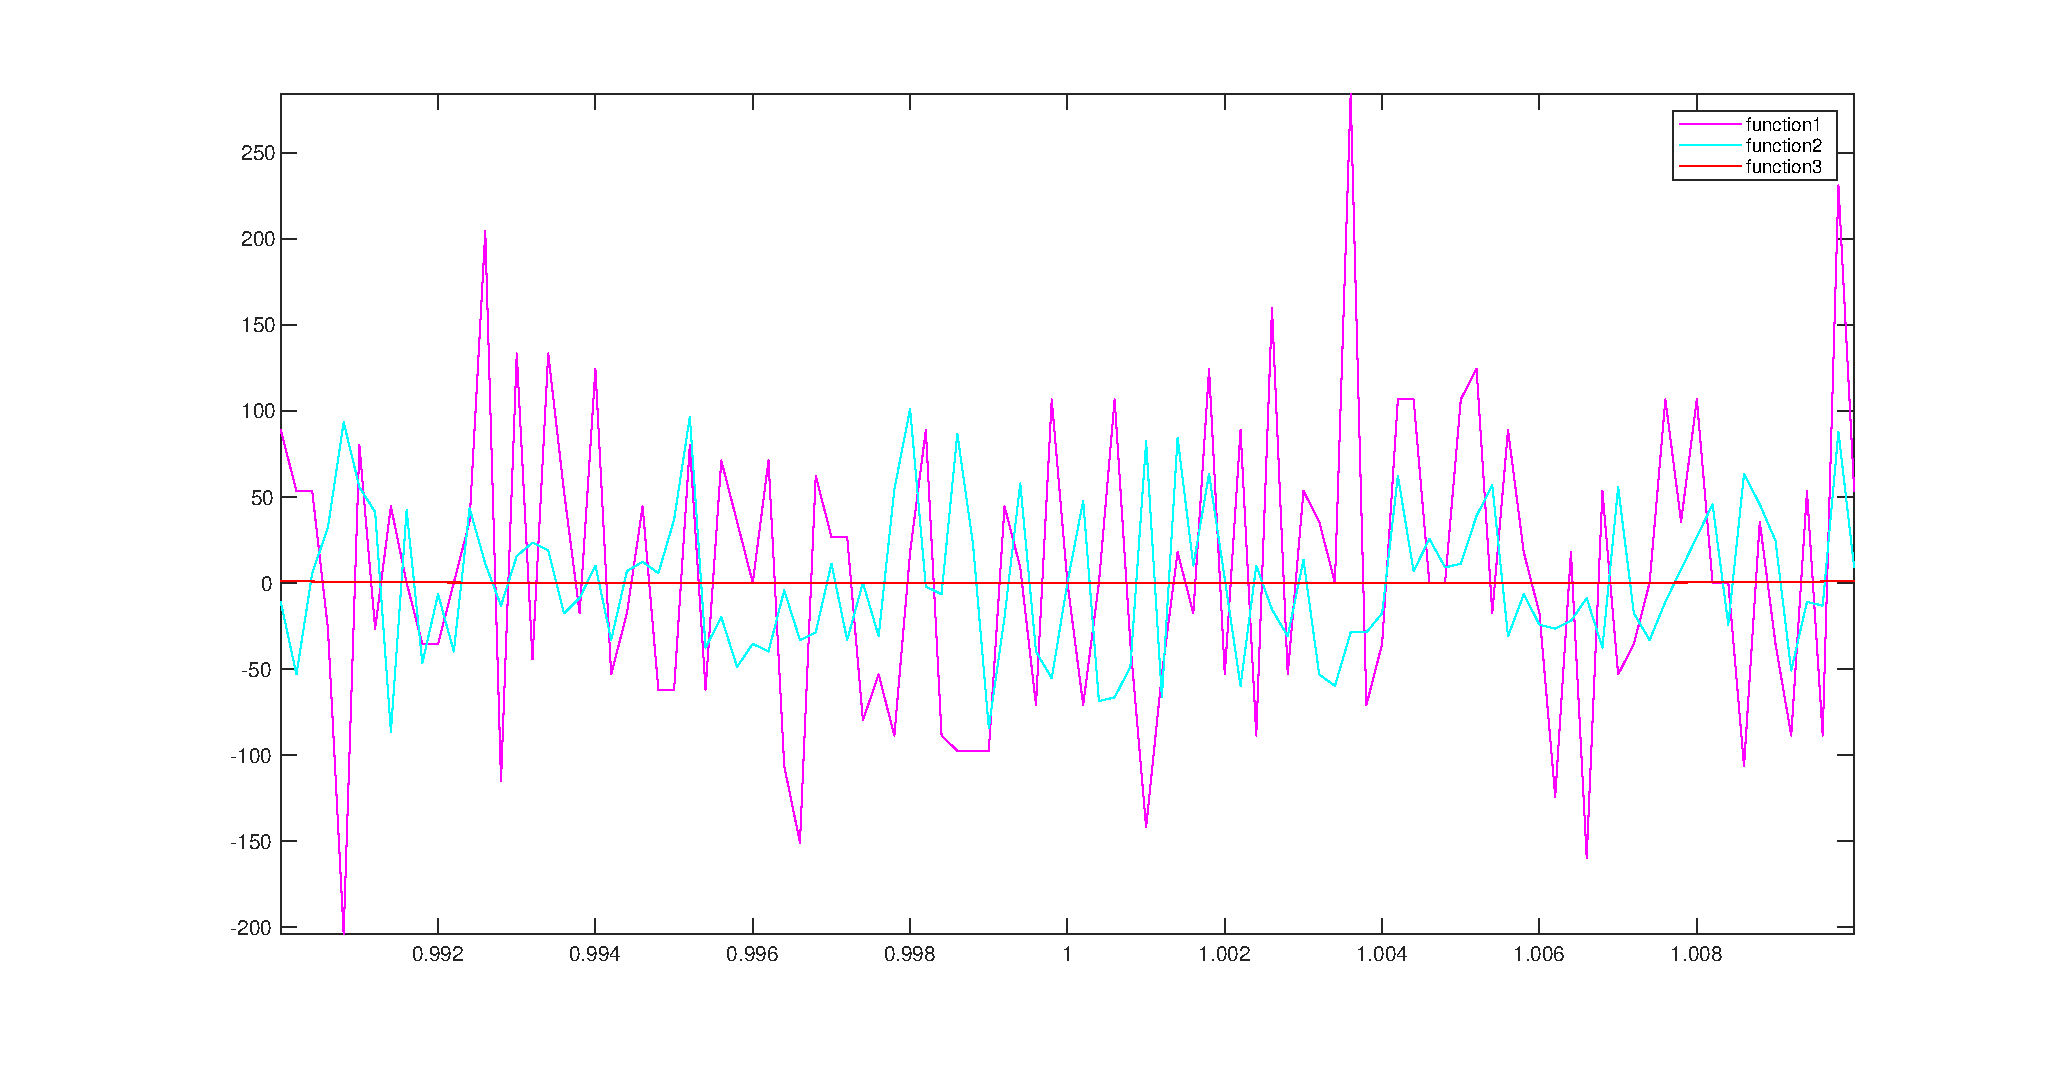
\includegraphics[width=15cm, height=7.5cm]{Plot1.eps}
        \caption{The values of each function multiplied by $10^{14}$.}
\end{figure} 
We can obviously found that the third function is the most accurate
, since it only use multiplication to calculate the result, which is accurate.
While the other two functions both uses addition and it causes catastrophic 
cancellation as the result is close to 0.


\section*{II. \small{Consider the normalized FPN system.}}

$UFL\left( \mathbb{F} \right)=0.5 $, $OFL\left( \mathbb{F} \right)= 3.5$.

\begin{figure}[ht]
        \centering
        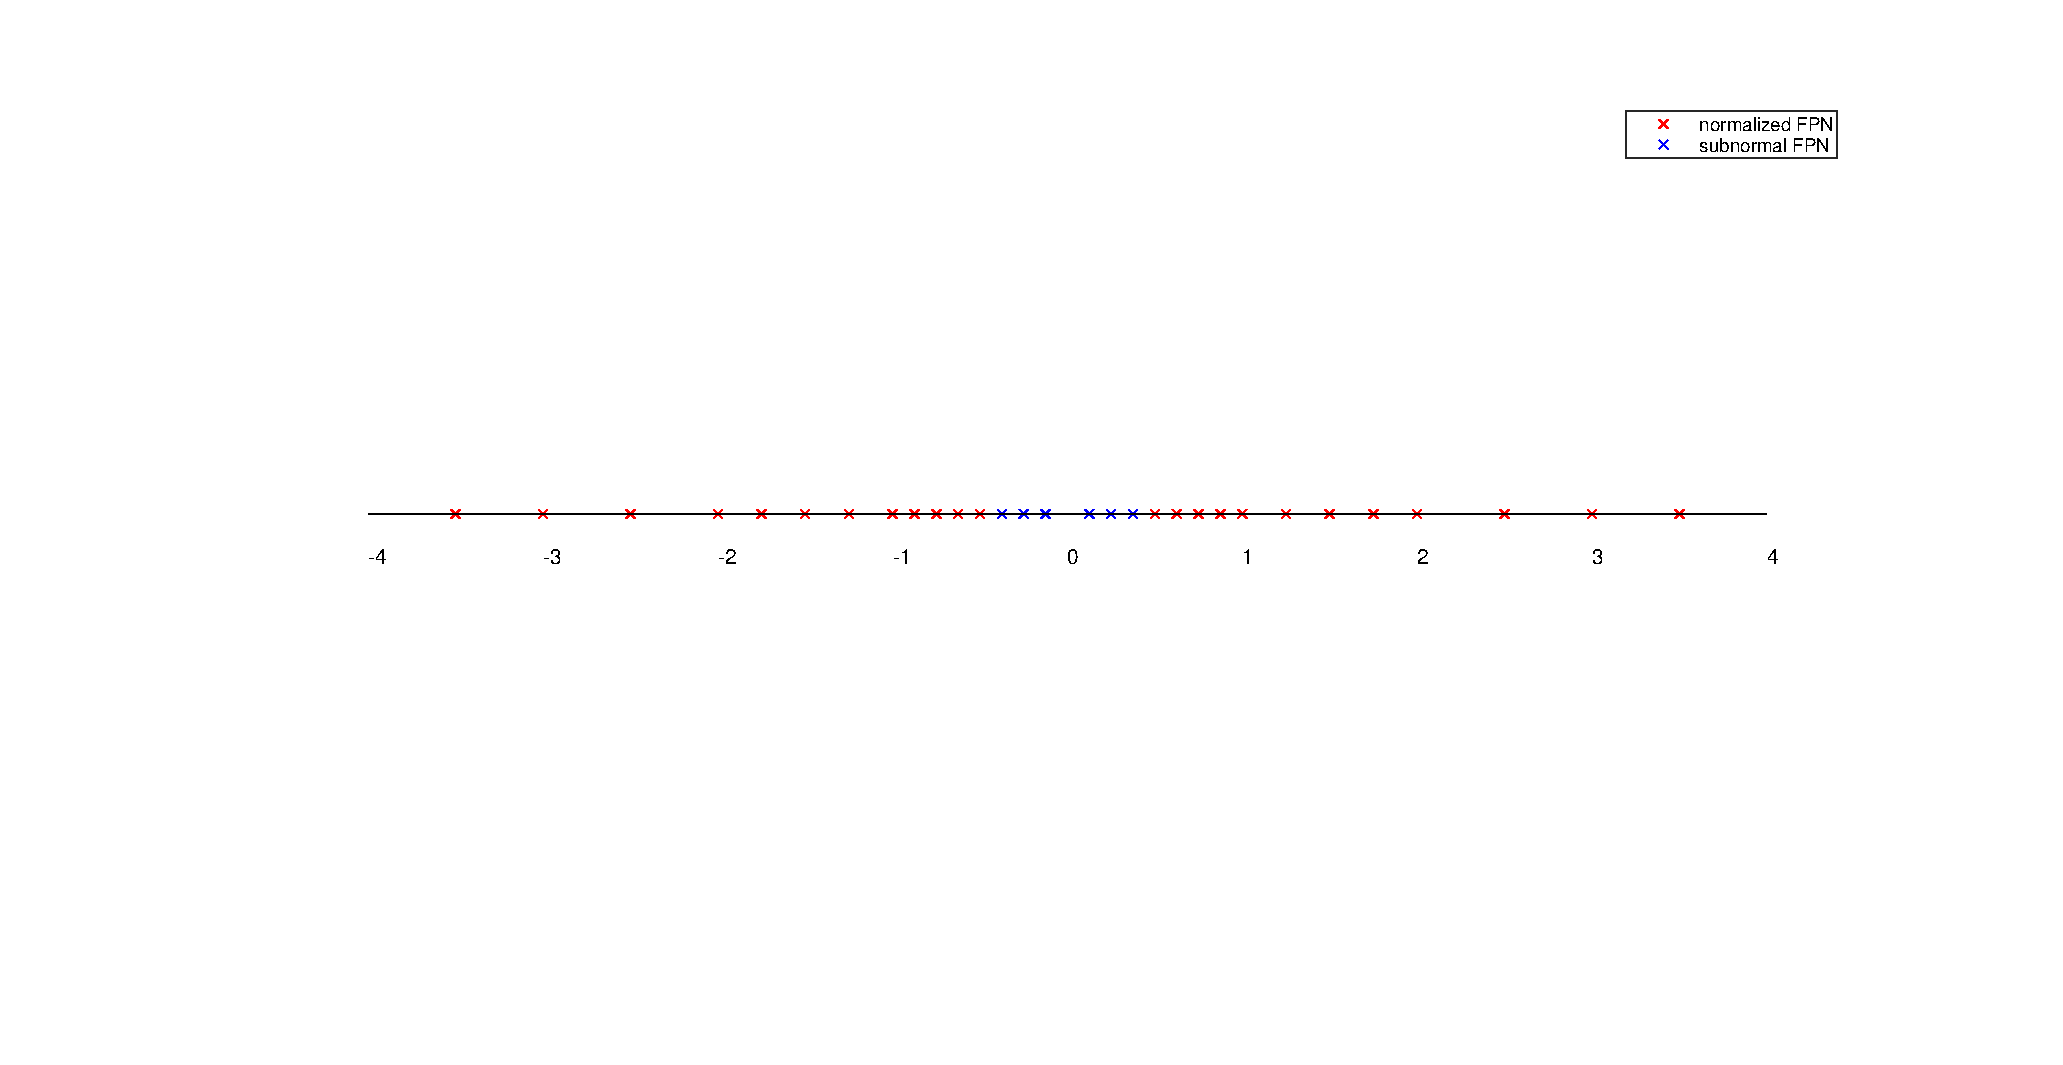
\includegraphics[width=15cm, height=7.5cm]{Plot2.eps}
	\caption{The normalized and subnormal numbers of $\mathbb{F}$}
\end{figure} 


\end{document}

%%% Local Variables: 
%%% mode: latex
%%% TeX-master: t
%%% End: 
